\begin{frame}	
	\frametitle{HTTP connection}
	\begin{columns}[t]
		\begin{column}[t]{0.5\linewidth}
			Http client:
			\begin{itemize}
				\item HttpURLConnection
				\item Custom-built client supports:
				\begin{itemize}
					\item cookies
					\item callbacks
					\item persistent settings					
				\end{itemize} 
				\item HttpAsyncTask class to run network operations independently from UI thread
				\item Implementation of an Android service to check requested video uploads
			\end{itemize}
		\end{column}
		\begin{column}[t]{0.5\linewidth}
			
			
		\end{column}		
	\end{columns}	
\end{frame}

\begin{frame}	
	\frametitle{Camera}
	\begin{columns}[t]
		\begin{column}[t]{0.5\linewidth}
			Camera:
			\begin{itemize}
				\item No use of phone's default camera application.
				\item SurfaceView class to display a preview: android.view.SurfaceView
				\item Android's MediaRecorder to record a video: android.media.MediaRecorder
				\item Storage of video files (.mp4 format) in the public directory for further usage. 
			\end{itemize}
		\end{column}
		\begin{column}[t]{0.5\linewidth}
			
			
		\end{column}		
	\end{columns}	
\end{frame}

\begin{frame}	
	\frametitle{Sensors}
	\begin{columns}[t]
		\begin{column}[t]{0.5\linewidth}
			Sensors:
			\begin{itemize}
				\item Accelerometer sensor for:
				\item Shake Detection
				\item Tilt Detection
				\item Preprocessed sensor data: ”Counter” value is sent to the server.
				\item Easy to add new sensors
			\end{itemize}
		\end{column}
		\begin{column}[t]{0.5\linewidth}
			
		\end{column}				
	\end{columns}	
\end{frame}

\begin{frame}	
	\frametitle{SQLite database}
	\begin{columns}[t]
		\begin{column}[t]{0.5\linewidth}
			SQLite database:
				\begin{itemize}
					\item Problem: coupling of actual video file and meta data persistently. 
					\item Use of Android's SQLite databases to have meta data persistently.
					\item Table: metadata
					\item Each filename is unique $\rightarrow$ column ``filename'' is handled as a foreign key to the actual video file.
				\end{itemize}
		\end{column}
		\begin{column}[t]{0.5\linewidth}
			
		\end{column}
	\end{columns}		
\end{frame}

\begin{frame}	
	\frametitle{SQLite database}
		Table metadata: \hrule
		\begin{description}	
			\item[id] int primary key
			\item[filename] text
			\item[timestamp] text
			\item[duration] int
			\item[width] int
			\item[height] int
			\item[shaking] int
			\item[tilt] int
			\item[serverId] int
			\item[status] int
		\end{description}
\end{frame}

\begin{frame}	
	\frametitle{User interface}
	\begin{columns}[t]
		\begin{column}[c]{.5\textwidth}
			\begin{figure}[!t]
				\centering
				\subfloat[Main]{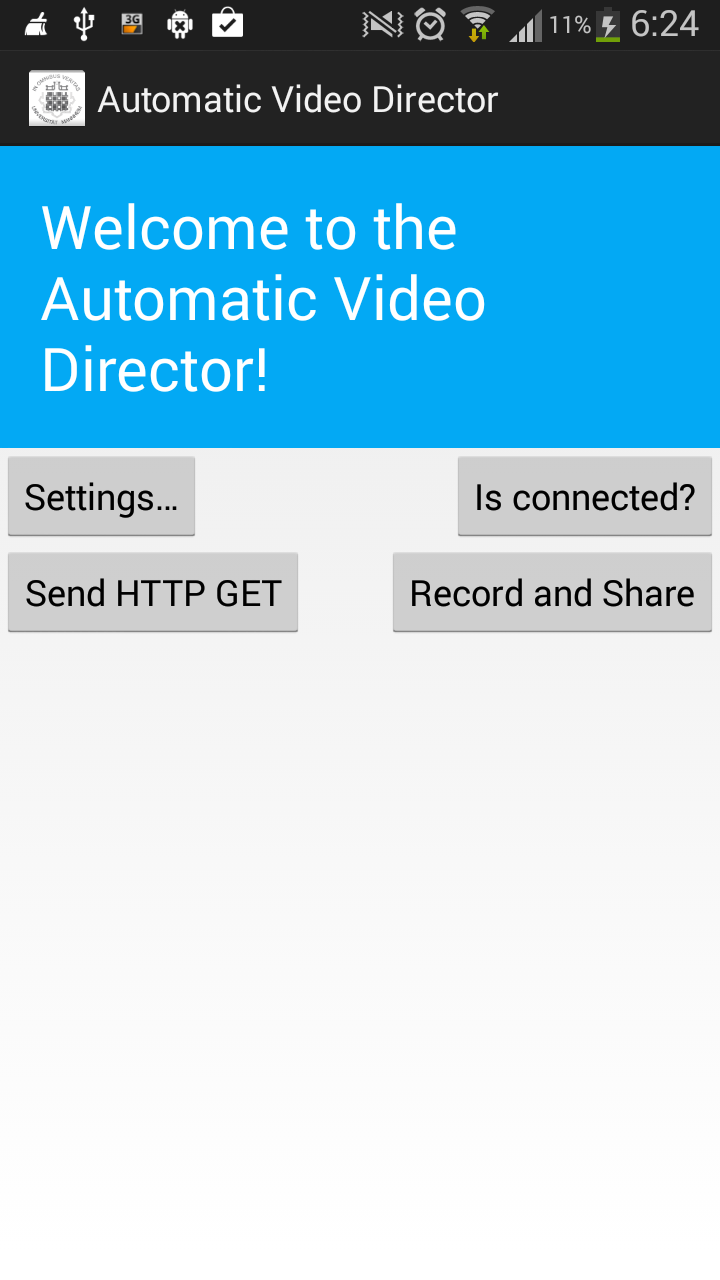
\includegraphics
						[width=.49\textwidth,height=.9\textheight,keepaspectratio]
						{ui_main.png}%
					\label{fig:ui_main}}
				\hfill
				\subfloat[Settings]{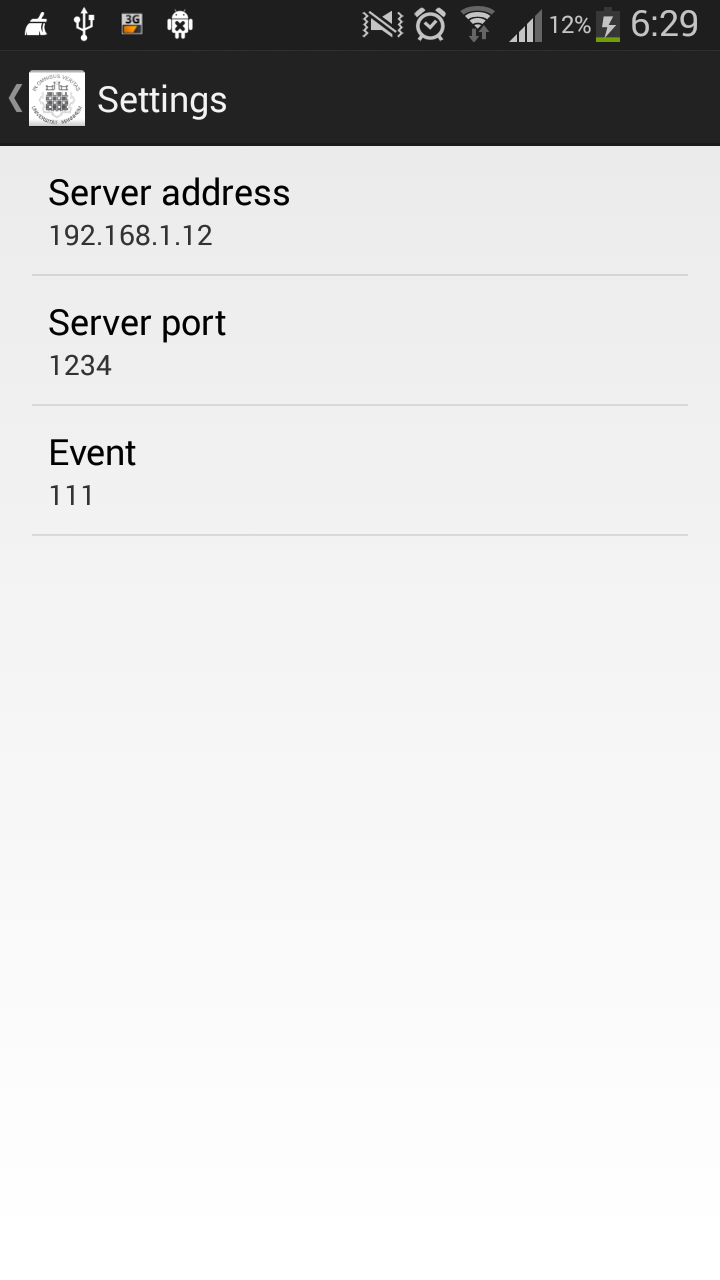
\includegraphics
					[width=.49\textwidth,height=.9\textheight,keepaspectratio]
					{ui_interface.png}%
					\label{fig:ui_settings}}
				\label{fig:ui_menu}
			\end{figure}
		\end{column}
		\begin{column}[c]{.5\textwidth}
			\begin{figure}[!t]
				\centering
				\subfloat[Camera]{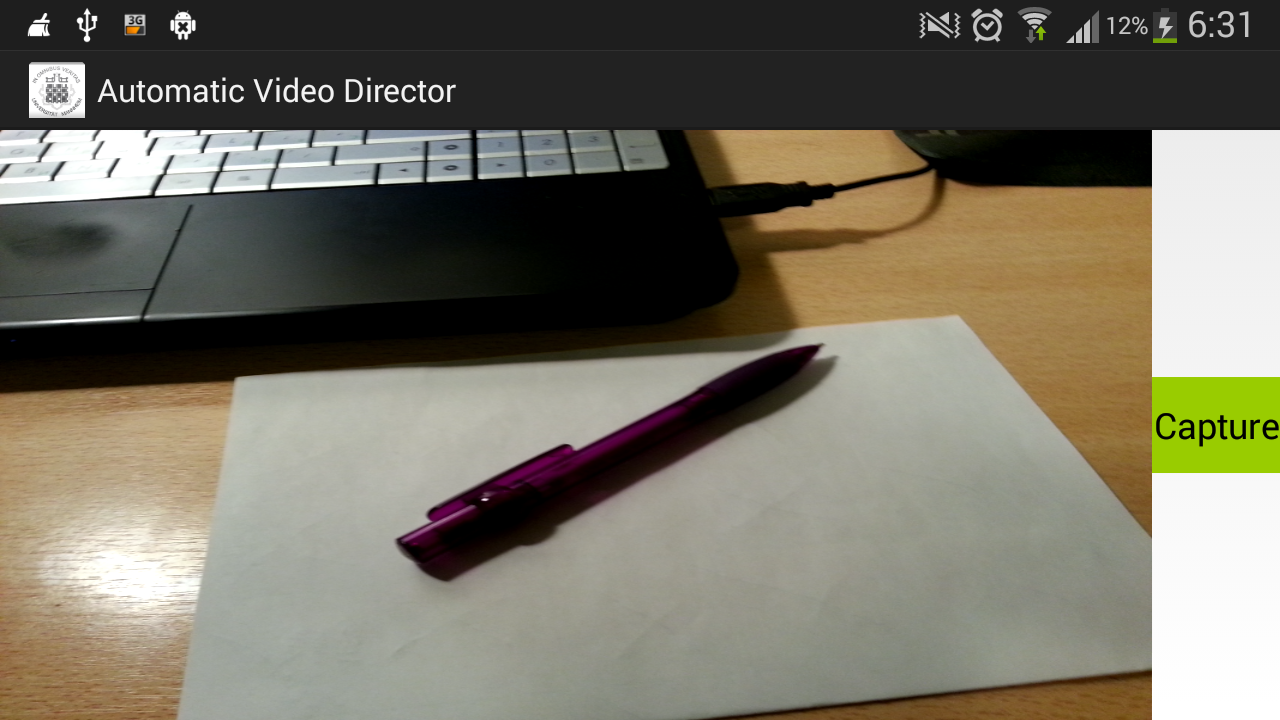
\includegraphics
					[width=\textwidth,height=.3\textheight,keepaspectratio]
					{ui_cam_green.png}%
					\label{fig:ui_cam_green}}
				\vfill
				\subfloat[Metadata upload]{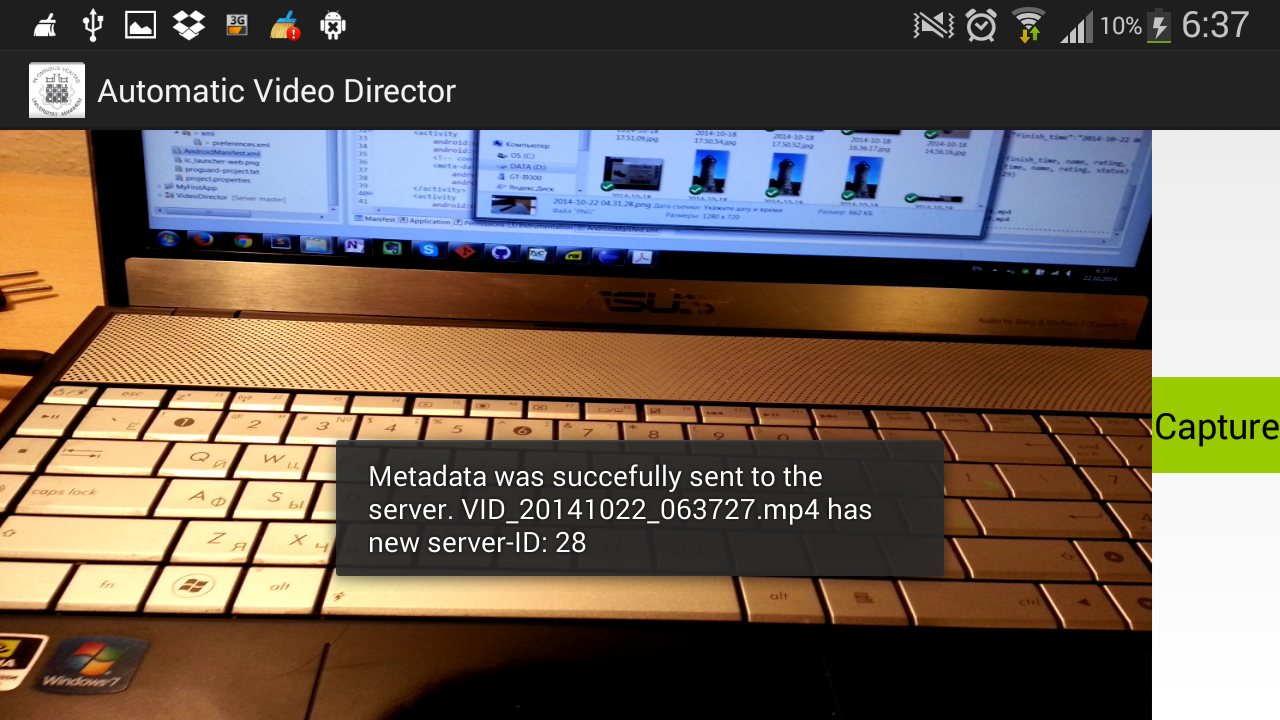
\includegraphics
					[width=\textwidth,height=.3\textheight,keepaspectratio]
					{ui_metadata.png}%
					\label{fig:ui_metadata}}
				\label{fig:ui_cam}
			\end{figure}
		\end{column}
	\end{columns}
\end{frame}